% !TeX root = main.tex
\documentclass[11pt,a4paper]{article}

% \documentclass[a4paper,14pt, draft]{article}

%%% отключение нумерации сраниц
\pagestyle{empty}
%%% значок в itemize
% \renewcommand{\labelitemi}{$\cdot$}

%%% Работа с русским языком
\usepackage{cmap}					% поиск в PDF
\usepackage{mathtext} 				% русские буквы в формулах
\usepackage[T1, T2A]{fontenc}			% кодировка %Т1 посоветовал чат гпт
\usepackage[utf8]{inputenc}			% кодировка исходного текста
\usepackage[english,russian]{babel}	% локализация и переносы
\usepackage{indentfirst}            % красная строка в первом абзаце
\frenchspacing                      % равные пробелы между словами и предложениями

%%% Дополнительная работа с математикой
\usepackage{amsmath,amsfonts,amssymb,amsthm,mathtools} % пакеты AMS
\usepackage{icomma}                                    % "Умная" запятая

%%% Свои символы и команды
\usepackage{centernot} % центрированное зачеркивание символа
\usepackage{stmaryrd}  % некоторые спецсимволы
\usepackage{dsfont}
\usepackage{amsthm}


\renewcommand{\epsilon}{\ensuremath{\varepsilon}}
\renewcommand{\phi}{\ensuremath{\varphi}}
\renewcommand{\kappa}{\ensuremath{\varkappa}}
\renewcommand{\le}{\ensuremath{\leqslant}}
\renewcommand{\leq}{\ensuremath{\leqslant}}
\renewcommand{\ge}{\ensuremath{\geqslant}}
\renewcommand{\geq}{\ensuremath{\geqslant}}
\renewcommand{\emptyset}{\ensuremath{\varnothing}}

\DeclareMathOperator{\sgn}{sgn}
\DeclareMathOperator{\ke}{Ker}
\DeclareMathOperator{\im}{Im}
\DeclareMathOperator{\re}{Re}

\newcommand{\N}{\mathbb{N}}
\newcommand{\Z}{\mathbb{Z}}
\newcommand{\Q}{\mathbb{Q}}
\newcommand{\R}{\mathbb{R}}
\newcommand{\Cm}{\mathbb{C}}
\newcommand{\F}{\mathbb{F}}
\newcommand{\id}{\mathrm{id}}
\newcommand{\imp}[2]{
	(#1\,\,$\ra$\,\,#2)\,\,
}
\newcommand{\Root}[2]{
	\left\{\!\sqrt[#1]{#2}\right\}
}
\newcommand{\RR}{\R}
\newcommand{\NN}{\N}
\renewcommand{\subseteq}{\subset}
\newcommand{\sub}{\subset}
\newcommand{\sconstr}{\;\vert\;}
\newcommand{\thus}{\implies}

\newcommand{\defeq}{\vcentcolon= }
\newcommand{\defev}{\stackrel{\Delta}{\Longleftrightarrow}}
\newcommand{\deriv}[3][1]{%
	\ifthenelse{#1>1}{%
		\frac{\dlta^{#1} {#2}}{\dlta {#3}^{#1}}
	}{%
		\frac{\dlta {#2}}{\dlta {#3}}
	}%
}

\renewcommand\labelitemi{$\triangleright$}

\let\bs\backslash
\let\lra\Leftrightarrow
\let\ra\Rightarrow
\let\la\Leftarrow
\let\emb\hookrightarrow

%%% Перенос знаков в формулах (по Львовскому)
\newcommand{\hm}[1]{#1\nobreak\discretionary{}{\hbox{$\mathsurround=0pt #1$}}{}}

%%% Работа с картинками
\usepackage{graphicx}    % Для вставки рисунков
\setlength\fboxsep{3pt}  % Отступ рамки \fbox{} от рисунка
\setlength\fboxrule{1pt} % Толщина линий рамки \fbox{}
\usepackage{wrapfig}     % Обтекание рисунков текстом

% \usepackage[inkscapeformat=png]{svg} %% svg

%%% Работа с таблицами
\usepackage{array,tabularx,tabulary,booktabs} % Дополнительная работа с таблицами
\usepackage{longtable}                        % Длинные таблицы
\usepackage{multirow}                         % Слияние строк в таблице

%%% Теоремы
\theoremstyle{plain}
\newtheorem*{theorem}{Теорема}
\newtheorem*{lemma}{Лемма}
\newtheorem*{proposition}{Утверждение}
\newtheorem*{exercise}{Упражнение}
\newtheorem*{problem}{Задача}

\theoremstyle{definition}
\newtheorem*{definition}{Определение}
\newtheorem*{corollary}{Следствие}
\newtheorem*{note}{Замечание}
\newtheorem*{reminder}{Напоминание}
\newtheorem*{example}{Пример}

\theoremstyle{remark}
\newtheorem*{solution}{Решение}

%%% Оформление страницы
\usepackage{extsizes}     % Возможность сделать 14-й шрифт
\usepackage{geometry}     % Простой способ задавать поля
\usepackage{setspace}     % Интерлиньяж
\usepackage{enumitem}     % Настройка окружений itemize и enumerate
\setlist{leftmargin=10pt} % Отступы в itemize и enumerate

\geometry{top=15mm}    % Поля сверху страницы
\geometry{bottom=5mm} % Поля снизу страницы
\geometry{left=10mm}   % Поля слева страницы
\geometry{right=10mm}  % Поля справа страницы

\setlength\parindent{15pt}        % Устанавливает длину красной строки 15pt
\linespread{1}                  % Коэффициент межстрочного интервала
%\setlength{\parskip}{0.5em}      % Вертикальный интервал между абзацами
\setcounter{secnumdepth}{0}      % Отключение нумерации разделов
%\setcounter{section}{-1}         % Нумерация секций с нуля
\usepackage{multicol}			  % Для текста в нескольких колонках
\usepackage{soulutf8}             % Модификаторы начертания
\mathtoolsset{showonlyrefs=true} % показывать номера формул только у тех, у которых есть ссылки по eqref
%%% Содержаниие
% \usepackage{tocloft}
% \tocloftpagestyle{main}
%\setlength{\cftsecnumwidth}{2.3em}
%\renewcommand{\cftsecdotsep}{1}
%\renewcommand{\cftsecpresnum}{\hfill}
%\renewcommand{\cftsecaftersnum}{\quad}

%%% Нумерация уравнений
\makeatletter
\def\eqref{\@ifstar\@eqref\@@eqref}
\def\@eqref#1{\textup{\tagform@{\ref*{#1}}}}
\def\@@eqref#1{\textup{\tagform@{\ref{#1}}}}
\makeatother                      % \eqref* без гиперссылки
\numberwithin{equation}{section}  % Нумерация вида (номер_секции).(номер_уравнения)
\mathtoolsset{showonlyrefs= true} % Номера только у формул с \eqref{} в тексте.

%%% Гиперссылки
\usepackage{hyperref}
\usepackage[usenames,dvipsnames,svgnames,table,rgb]{xcolor}
\hypersetup{
	unicode=true,            % русские буквы в раздела PDF
	colorlinks=true,       	 % Цветные ссылки вместо ссылок в рамках
	linkcolor=black!15!blue, % Внутренние ссылки
	citecolor=green,         % Ссылки на библиографию
	filecolor=magenta,       % Ссылки на файлы
	urlcolor=NavyBlue,       % Ссылки на URL
}

%%% Графика
\usepackage{tikz}        % Графический пакет tikz
\usepackage{tikz-cd}     % Коммутативные диаграммы
\usepackage{tkz-euclide} % Геометрия
\usepackage{stackengine} % Многострочные тексты в картинках
\usetikzlibrary{angles, babel, quotes}
\title{\texttt{Измерение вязкости воздуха по течению в тонких трубках \\ 2.2.1}}
\author{}
\date{}

\begin{document}

\maketitle

\textbf{Цель работы:} экспериментально исследовать свойства течения газов по тонким трубкам при различных числах Рейнольдса; выявить область применимости закона Пуазейля и с его помощью определить коэффициент вязкости воздуха.

\textbf{В работе используются:} система подачи воздуха (компрессор, поводящие трубки); газовый счетчик барабанного типа; спиртовой микроманометр с регулируемым наклоном; 
набор трубок различного диаметра с выходами для подсоединения микроманометра; секундомер

\section*{\texttt{Теория}}

Работа посвящена изучению течения воздуха по прямой трубе круглого сечения. Движение жидкости или газа вызывается перепадом внешнего давления на концах $\Delta P$ трубы, чему в свою очередь препятствуют силы вязкого (внутреннего) трения, действующие между соседними слоями жидкости, а также со стороны стенок трубы.

Сила вязкого трения как в жидкостях, так и в газах описывается законом
Ньютона: касательное напряжение между слоями пропорционально перепаду
скорости течения в направлении, поперечном к потоку. В частности, если жидкость течёт вдоль оси x,  а скорость течения $v_{x}(y)$ зависит от координаты $y$  в каждом слое возникает направленное по $x$ касательное напряжение.
\[\tau_{xy} = -\eta \frac{\partial v_x}{\partial y}\]
Величину $\eta$ называют коэффициентом динамической вязкости (или просто вязкостью) среды.

Объёмным расходом (или просто расходом) $Q$ называют объём жидкости,
протекающий через сечение трубы в единицу времени. Величина $Q$ зависит от
перепада давления $\Delta P$, а также от свойств газа (плотности $\rho$ и вязкости $\eta$) и от
геометрических размеров (радиуса трубы $R$ и её длины $L$). Основная задача
данной работы — исследовать эту зависимость экспериментально.

Характер течения в трубе может быть ламинарным либо турбулентным. 

Характер течения определяется безразмерным параметром задачи — числом Рейнольдса

$$ Re = \frac{\rho u a}{\eta}$$ 

где $\rho$ - плотность жидкости, $u$ - скорость движения потока, $a$ - характерный размер потока.

Вспомним уравнения, изучавшиеся в первом семестре:

% $$P(x) = P_{0} - \frac{\Delta P}{l}x$$ (очевидно)

$$u = \frac{Q}{\pi R^{2}} = \frac{u_{max}}{2}$$ (средняя скорость потока)

$$Q = \frac{\pi R^{4} \Delta P}{8\eta l}$$ (Формула Пуазейля)

$$l_{\text{уст}} \approx 0,2R\cdot Re$$ (коэффицент получен экспериментально)
\newpage

\section*{\texttt{Установка}}

\begin{figure}[h!]
	\begin{center}
		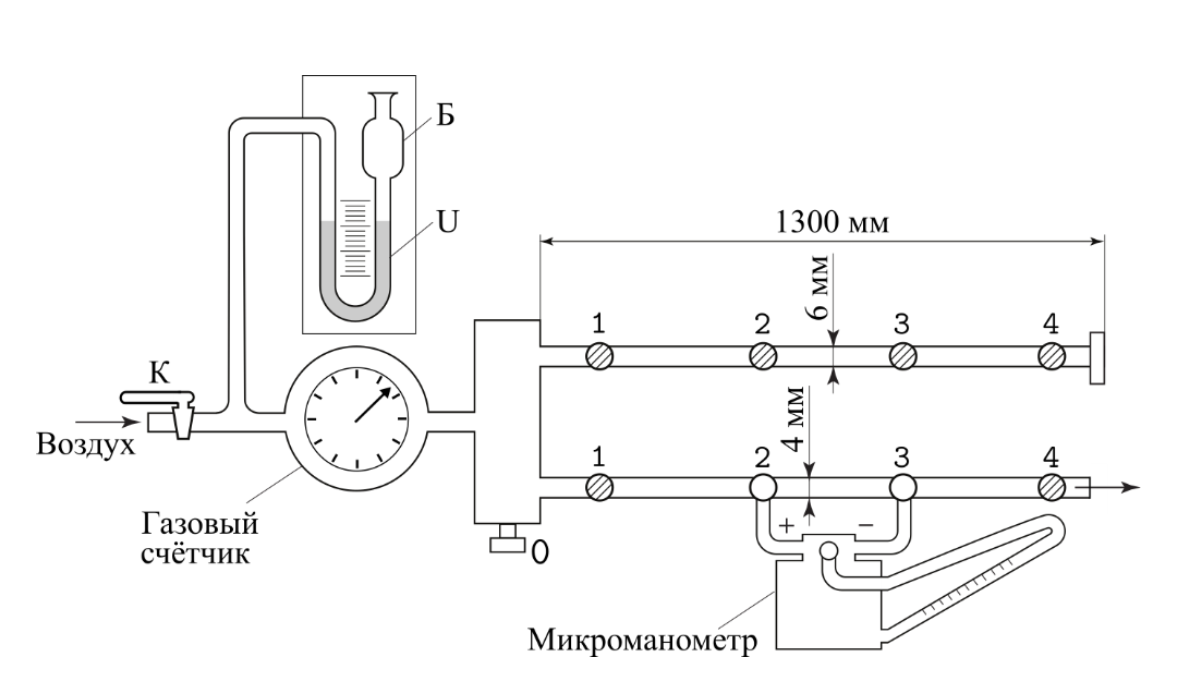
\includegraphics[width = 0.9\textwidth]{ust}
		\caption{Схема экспериментальной установки}
		\label{fig:facility}
	\end{center}
\end{figure}

\section{\textbf{Ход работы}}
\begin{enumerate}
\item Зафиксируем в параметры экспериментальной установки:
\begin{table}[h!]
  \centering
  \begin{tabular}{|c|c|c|}
  \hline
  Участок трубки & $l$, см & $\sigma$, мм \\ \hline
  1                 & 11      & 1            \\ \hline
  2                 & 30      & 1            \\ \hline
  3                 & 40      & 1            \\ \hline
  4                 & 50      & 1            \\ \hline
  \end{tabular}
  \caption{Длины участков второй трубки между различными точками подключения.}
  \label{tab:second_tube_parametrs}
\end{table}

\begin{table}[h!]
\centering
\begin{tabular}{|c|c|c|}
\hline
              & $d$, мм & $\sigma$, мм \\ \hline
Первая трубка & 5,25    & 0,05         \\ \hline
Вторая трубка & 3,90    & 0,05         \\ \hline
\end{tabular}
\caption{Внутренние диаметры трубок установки}
\label{tab:facilitys_tube_diam}
\end{table}

\item Проведем измерение зависимости разности давлений от расхода воздуха. 
Для этого будем отмерять объём воздуха, занимающий целое число шкал (для удобсвта) проходящий через газовый счетчик и засекать продолжительность замера. 
Результаты занесем в таблицу 3.
 
\begin{table}[h!]
\centering
\begin{tabular}{|c|c|c|c|c|c|c|c|}
\hline
№ измерения & $\Delta h$, дел & $\Delta V$, л & $\delta V$, л & $t_{1}$, с & $t_{2}$, с & $t_{3}$, с & $t_{4}$, с \\ \hline
1           & 34              & 5             & 0,05          & 102,8      & 103,1      & 102,95     & 102,9      \\ \hline
2           & 58              & 5             & 0,05          & 74,5       & 74,8       & 74,3       & 74,4       \\ \hline
3           & 65              & 5             & 0,05          & 57,5       & 57,54      & 57,63      & 57,89      \\ \hline
4           & 86              & 5             & 0,05          & 50,36      & 50,76      & 51,17      & 51,34      \\ \hline
5           & 125             & 5             & 0,05          & 45,02      & 45,2       & 45,11      & 45,33      \\ \hline
6           & 166             & 5             & 0,05          & 39,69      & 39,08      & 39,5       & 39,44      \\ \hline
7           & 212             & 5             & 0,05          & 34,75      & 34,28      & 34,92      & 34,65      \\ \hline
8           & 257             & 7,5           & 0,05          & 46,8       & 46,89      & 48,91      & 46,95      \\ \hline
\end{tabular}
\caption{Результаты измерения зависимости перепада давления от расхода воздуха между точками 2 - 3 второй трубки}
\label{tab:flow_measuring_2_3_second_tube}
\end{table}

\begin{table}[h!]
\centering
\begin{tabular}{|c|c|c|c|c|c|c|c|}
\hline
№ измерения & $\Delta h$, дел & $\Delta V$, л & $\delta V$, л & $t_{1}$, с & $t_{2}$, с & $t_{3}$, с & $t_{4}$, с \\ \hline
1           & 25              & 5             & 0,2           & 171,31     & 171,98     & 170,64     & 171,57     \\ \hline
2           & 55              & 5             & 0,2           & 80,95      & 81,34      & 81,12      & 80,76      \\ \hline
3           & 95              & 5             & 0,2           & 54,96      & 55,01      & 55,23      & 54,81      \\ \hline
4           & 120             & 5             & 0,2           & 49,82      & 49,48      & 49,33      & 49,23      \\ \hline
5           & 150             & 5             & 0,2           & 45,04      & 44,64      & 45,01      & 44,95      \\ \hline
6           & 180             & 5             & 0,2           & 41,79      & 41,57      & 41,83      & 42,38      \\ \hline
7           & 210             & 5             & 0,2           & 39,08      & 38,59      & 38,63      & 38,65      \\ \hline
8           & 240             & 5             & 0,2           & 36,57      & 36,1       & 36,16      & 36,42      \\ \hline
\end{tabular}
\caption{Результаты измерения зависимости перепада давления от расхода воздуха между точками 3 - 4 второй трубки}
\label{tab:flow_measuring_3_4_second_tube}
\end{table}

\item Построим графики по этим таблицам:

\begin{figure}[h!]
	\begin{center}
		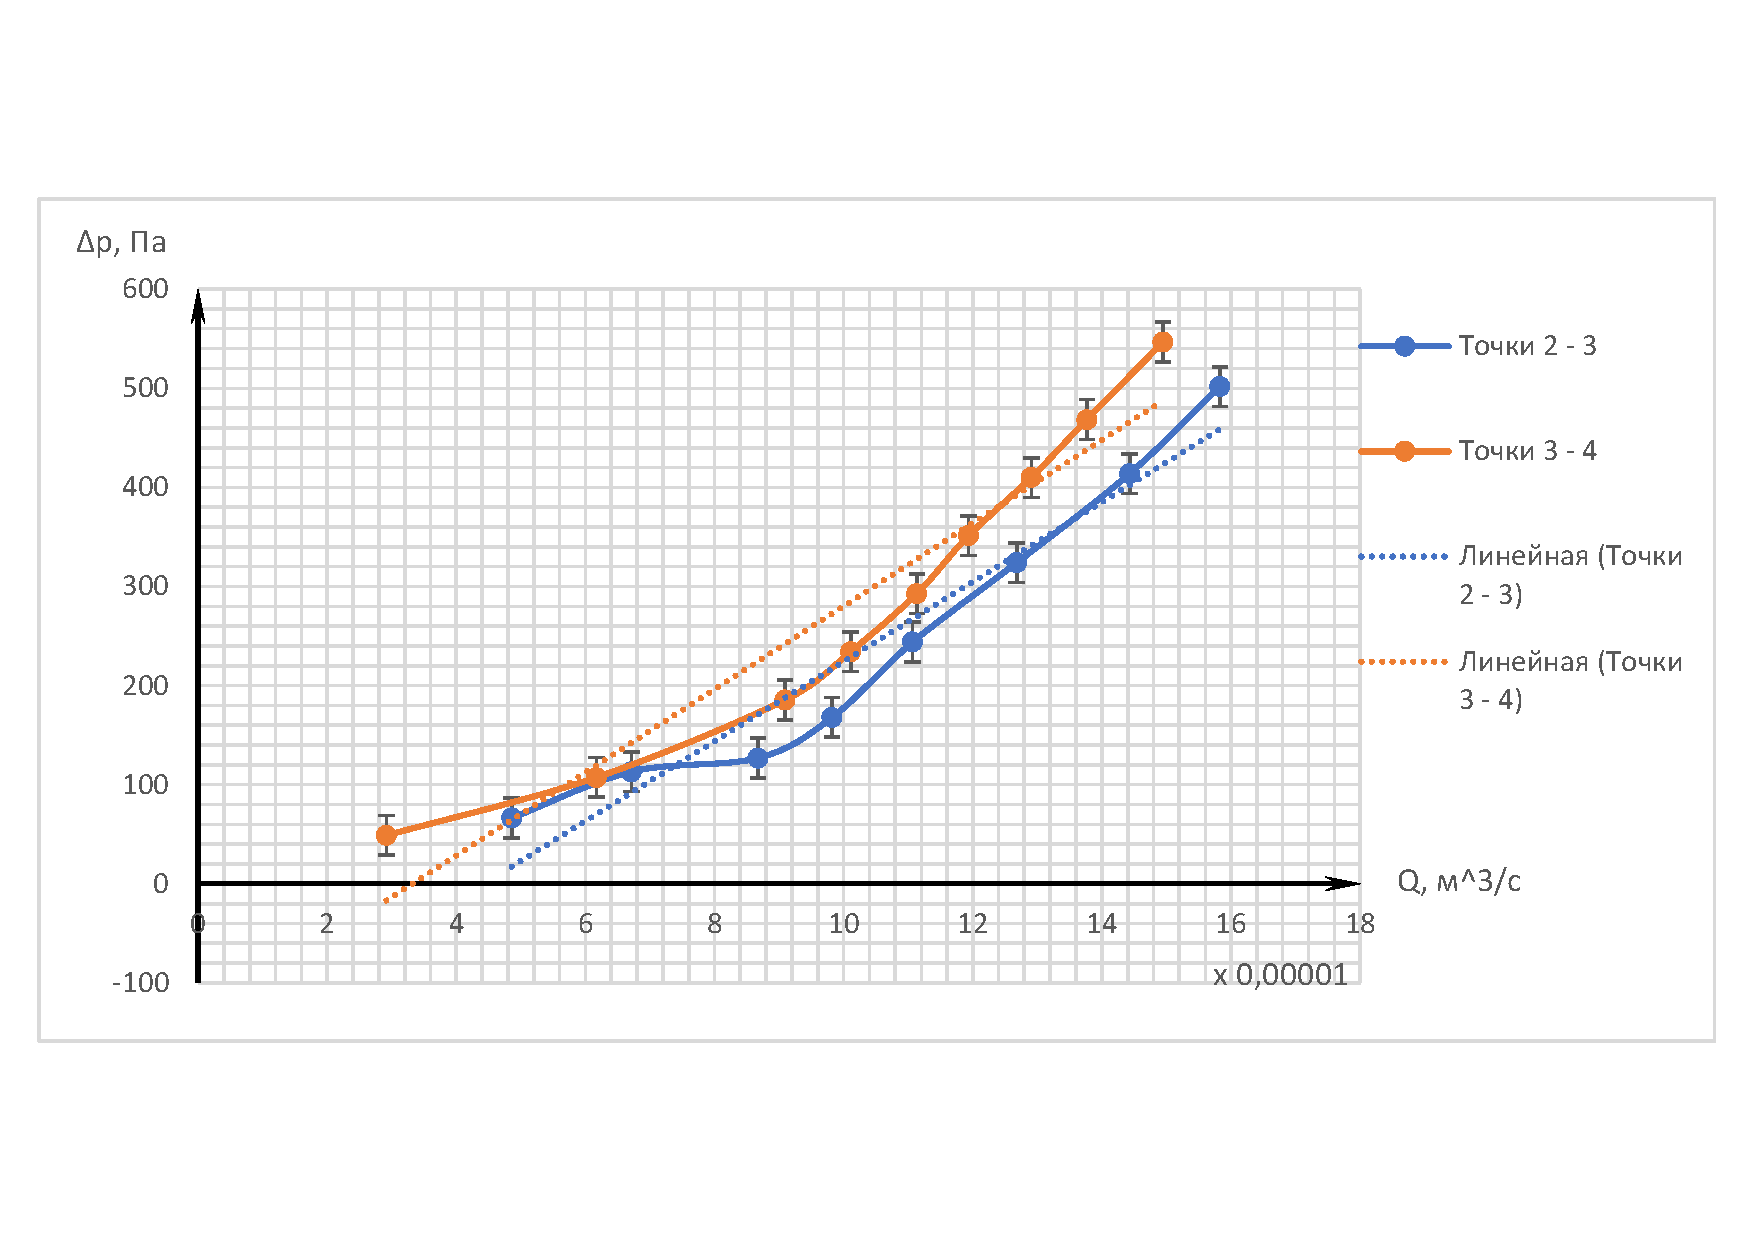
\includegraphics[width = 0.85\textwidth]{Results_of_measuring}
		\caption{графики зависимости перепада давления от расхода воздуха для второй трубки и точек 2 - 3, 3 - 4}
		\label{fig:graph_1}
	\end{center}
\end{figure}

\item Через МНК определим значение и погрешность вязскости воздуха.

\begin{table}[]
\centering
\begin{tabular}{|c|c|c|c|c|c|c|c|}
\hline
$ \Delta P $, Па & $ \sigma_{\Delta P} $, Па & $ Q \cdot 10^{5} \quad \frac{\text{м}^{3}}{\text{с}}$ & $\sigma_{Q}\cdot 10^5 \quad \frac{\text{м}^{3}}{\text{с}} $ & $ \Delta P $, Па & $ \sigma_{\Delta P} $, Па & $ Q \cdot 10^{5} \quad \frac{\text{м}^{3}}{\text{с}}$ & $\sigma_{Q}\cdot 10^5 \quad \frac{\text{м}^{3}}{\text{с}} $ \\ \hline
66             & 2                       & 4,857                                          & 0,005                                                  & 49                              & 22                  & 2,92           & 0,01                   \\ \hline
113            & 4                       & 6,711                                          & 0,007                                                  & 107                             & 10                  & 6,17           & 0,02                   \\ \hline
127            & 4                       & 8,675                                          & 0,009                                                  & 185                             & 7                   & 9,09           & 0,04                   \\ \hline
168            & 9                       & 9,822                                          & 0,010                                                  & 234                             & 10                  & 10,11          & 0,04                   \\ \hline
244            & 3                       & 11,071                                         & 0,011                                                  & 293                             & 7                   & 11,13          & 0,04                   \\ \hline
324            & 5                       & 12,682                                         & 0,013                                                  & 351                             & 14                  & 11,94          & 0,05                   \\ \hline
414            & 5                       & 14,430                                         & 0,014                                                  & 410                             & 9                   & 12,91          & 0,05                   \\ \hline
502            & 20                      & 15,827                                         & 0,011                                                  & 469                             & 9                   & 13,77          & 0,06                   \\ \hline
\multicolumn{4}{|c|}{}                                                                                                                             & 547                             & 8                   & 14,95          & 0,00                   \\ \hline
\end{tabular}
\caption{Результаты измерения перепадов давления, расхода, а также погрешности данных измерений}
\label{tab:flow_and_delta_with_mistakes}
\end{table}

Исходя из полученных данных, выбирая наиболее линейные участки на графиках, получим с помощью МНК значение вязкости воздуха, определенное по формуле Пуазейля:

$$\eta = 1,9 \cdot 10^{-6}; \quad \sigma_{\eta} = 6 \cdot 10^{-7},$$

$$\eta = \left(1,9 \pm 0,6 \right)\cdot 10^{-6} \text{Па}\cdot\text{c} $$

Построим графики зависимости падения давления от длины трубки (\ref{fig:graph_2}).

\begin{figure}[h!]
	\begin{center}
		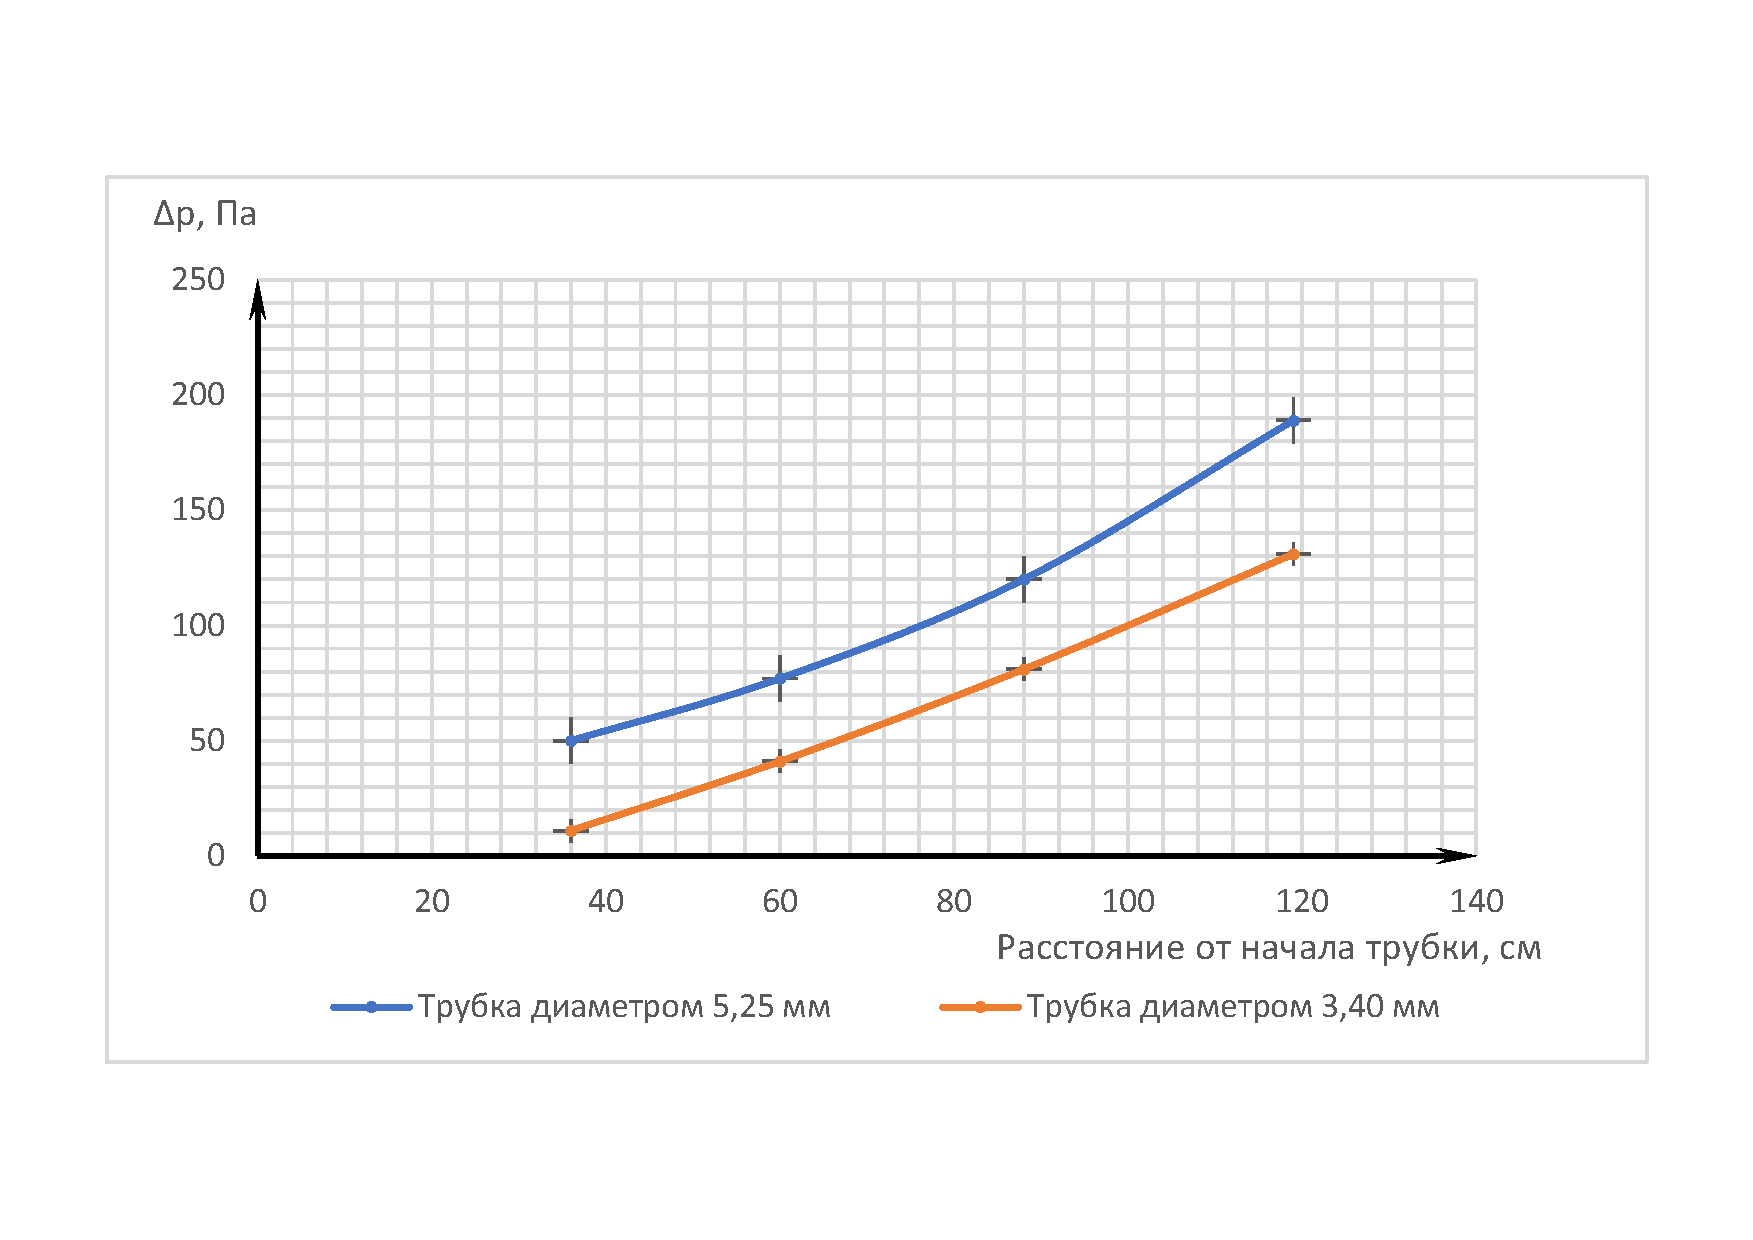
\includegraphics[width = 0.85\textwidth]{graph_2}
		\caption{графики зависимости перепада давления от расстояния до начала трубки}
		\label{fig:graph_2}
	\end{center}
\end{figure}


\end{enumerate}
\section{Вывод}

\begin{enumerate}
	\item При выполнении данной работы были исследованы различные режимы течения газа по трубкам. На практике получена экспериментальная зависимость разницы давления в различных точках трубки в зависимости от расхода воздуха, идущего через трубку.
	\item Исследовались условия перехода течения из одного режима (ламинарного) в другой (турбулентный).
	\item Полученные зависимости разницы давлений от расхода воздуха согласуются с существующей теорией, описывающей движение газов и жидкостей в различных режимах.
	\item Определено значение вязкости воздуха : $\eta_{\text{эксп}} = \left(1,9 \pm 0,6\right) \cdot 10^{-6}$ Па$\cdot$с, при табличном значении $\eta_{\text{табл}} = \left(1,3 \pm 0,2\right) \cdot 10^{-6}$ Па$\cdot$с. Полученные значения равны в пределах погрешности.
	\item Основной вклад в погрешность итогового значения вязкости внесла погрешность измерения времени, а так же погрешности измерения давлений. Погрешности, связанные с установкой (погрешность линейных размеров установки, диаметра трубок) внесли меньший вклад в итоговое значение погрешности.
	\item Частично подтверждена теоретическая линейная зависимость падания давления с изменением расстояния от края трубки.
	\item Подтверждена формула Пуазейля для расхода газа при прохождении через трубку.
\end{enumerate}
\end{document}